\subsection{\hmath $W[2]$-hard on Bipartite Graphs}

\begin{definition}[Bipartite Graph, {\cite[p.5]{Bondy2008}}]
    
A \textit{\bg} is a Graph G whose vertex set can be partitioned into two subsets X and Y, so that each edge has one end in X and one end in Y. Such a partition (X,Y) is called a \textit{bipartition} of G.

\end{definition}

\begin{figure}[htb]
    \centering
\definecolor{myblue}{RGB}{80,80,160}
\definecolor{mygreen}{RGB}{80,160,80}

\resizebox{0.9\textwidth}{!}{
\begin{tikzpicture}[thick,
        every node/.style={draw,circle},
        fsnode/.style={fill=myblue},
        ssnode/.style={fill=mygreen},
        every fit/.style={ellipse,draw,inner sep=-2pt,text width=2.2cm},
        -,shorten >= 3pt,shorten <= 3pt
    ]
    % the vertices of U
    \begin{scope}[xshift=2cm,start chain=going below, node distance=7mm]
        \foreach \i in {1,2,...,5}
        \node[fsnode,on chain] (f\i) [label=above left: $x_\i$] {};
    \end{scope}

    \begin{scope}[start chain=going below, node distance=7mm]
        \foreach \i [count=\j] in {6,7,...,10}
        \node[ssnode,on chain] (f\i) [label=above left: $x'_{\j}$] {};
    \end{scope}

    % the vertices of V
    \begin{scope}[xshift=5cm,yshift=-0.5cm,start chain=going below, node distance=7mm]
        \foreach \i [count=\j] in {11,12,...,14}
        \node[ssnode,on chain] (f\i) [label=above right: $y_{\j}$] {};
    \end{scope}
    
    \begin{scope}[xshift=7cm,yshift=-0.5cm,start chain=going below, node distance=7mm]
        \foreach \i [count=\j] in {15,16,...,18}
        \node[fsnode,on chain] (f\i) [label=above right: $y'_{\j}$] {};
    \end{scope}

    \node [fsnode, left=of f8, xshift=-1cm] (nx) [label=above left: $d_1$]{};
    \node [ssnode, right=of nx, xshift=11cm] (ny) [label=above right: $d_2$]{};

    \node [ssnode, left=of nx] (nxx) [label=left: $u_1$]{};
    \node [fsnode, right=of ny] (nyy) [label=right: $u_2$]{};

    % the set U
    \node [myblue,fill=aqua, opacity=0.1,fit=(f1) (f5),label=above:$X$] {};
    \node [mygreen,fill=applegreen, opacity=0.1,fit=(f11) (f14),label=above:$Y$] {};

    \node [mygreen,fill=applegreen, opacity=0.1, fit=(f6) (f10),label=above:$ $] {};
    \node [myblue,fill=aqua, opacity=0.1, fit=(f18) (f15),label=above:$ $] {};
     
    % the set V
    % \node [mygreen,fit=(s6) (s9),label=above:$V$] {};

    % the edges
    \draw (f1) -- (f11);
    \draw (f1) -- (f12);
    \draw (f1) -- (f14);
    \draw (f2) -- (f14);
    \draw (f3) -- (f13);
    \draw (f3) -- (f11);
    \draw (f5) -- (f12);
    \draw (f4) -- (f14);
    
    \foreach \i in {6,7,...,10}
    \draw (nx) -- (f\i);

    \foreach \i in {15,16,...,18}
    \draw (ny) -- (f\i);

    \draw (ny) -- (nyy);
    \draw (nx) -- (nxx);

    % The doubled edges
    \draw (f6) -- (f1);
    \draw (f7) -- (f2);
    \draw (f8) -- (f3);
    \draw (f9) -- (f4);
    \draw (f10) -- (f5);

    \draw (f11) -- (f15);
    \draw (f12) -- (f16);
    \draw (f13) -- (f17);
    \draw (f14) -- (f18);

\end{tikzpicture}
}
\caption{Constructing G' from a bipartite Graph G by duplicating the vertices and adding a dominating tail}
\end{figure}


\begin{theorem}
    Semitotal Dominating Set is $\omega[2]$ hard for bipartite Graphs
\end{theorem}

\begin{proof}
    Given a bipartite Graph $G = ( \{X \cup Y\}, E)$, we construct a bipartite Graph G' in the following way:
    \begin{enumerate}
        \item For each vertex $x_i \in X$ we add a new vertex $x_i'$  and an edge $(x_i, x_i')$ in between.
        \item For each vertex $y_j \in Y$ we add a new vertex $y_j'$ and an edge $(y_j, y_j')$ in between.
        \item We add two $P_1$, namely $(u_1, d_1)$ and $(u_2, d_2)$, and connect them with all $(d_1, x_i')$ and $(d_2, y_j')$ respectively.
    \end{enumerate}
    \paragraph*{Observation:} G' is clearly bipartite as all $y'_j$ and $x'_i$ form again an Independent Set. Setting  $X' = X \cup \{u_2\} \cup \bigcup y'_i$ and $Y' = Y \cup \{u_1\} \cup \bigcup {x'_i}$ form the partitions of bipartite G'.

    \begin{corollary} G has a Dominating Set of size k iff G has a Semitotal Dominating Set of size $k' = k + 2$
    \end{corollary} 
    $\Rightarrow$: Asume there exists a Dominating Set D in G with size k. $DS = D\cup \{d_1,d_2\}$ is a Semitotal Dominating Set in $G'$ with size $k' = k+2 $ , because $d_1$ dominates $u_1$ and all $x'_i$; $d_2$ dominates $u_2$ and all $y'_i$. Hence, it is a Semitotal Dominating Set, because $\forall v \in (D \cap X): d(v, d_1) = 2$ and $\forall v \in (D \cap Y): d(v, d_2) = 2$

    $\Leftarrow$: On the contrary, asume any Semitotal Dominating Set $SD$ in $G'$ with size $k'$. WLOG we can asume that $u_1, u_2 \notin DS$. 
    
    Our construction forces $d_1$, $d_2 \in DS$. Because all $x'_i$ are only important in dominating $x_i$ ($y'_i$ for $y_i$ resp.) as $d_1, d_2 \in DS$. If $x'_i \in DS$ we simply exchange it with $x_i$ (for $y'_i$ and $y_i$ respectively) in our DS keeping the size of the dominating set. $D = DS \setminus \{ d_1,d_2\}$ give us a Dominating Set in G with size $ k = k' - 2$

    As G' can be constructed in $\mathcal{O}(n)$ and parameter k is only blown up by a constant, this reduction is a FPT reduction. As Dominating Set is $w[2]$ hard for bipartite Graphs\footnote{Citation needed!} so is Semitotal Dominating Set.
\end{proof}

\subsection{\hmath $W[2]$-hard on Chordal Graphs}
\begin{theorem}
    Semitotal Dominating Set is $\omega[2]$ hard on Chordal Graphs
\end{theorem}

\begin{figure}[th]
    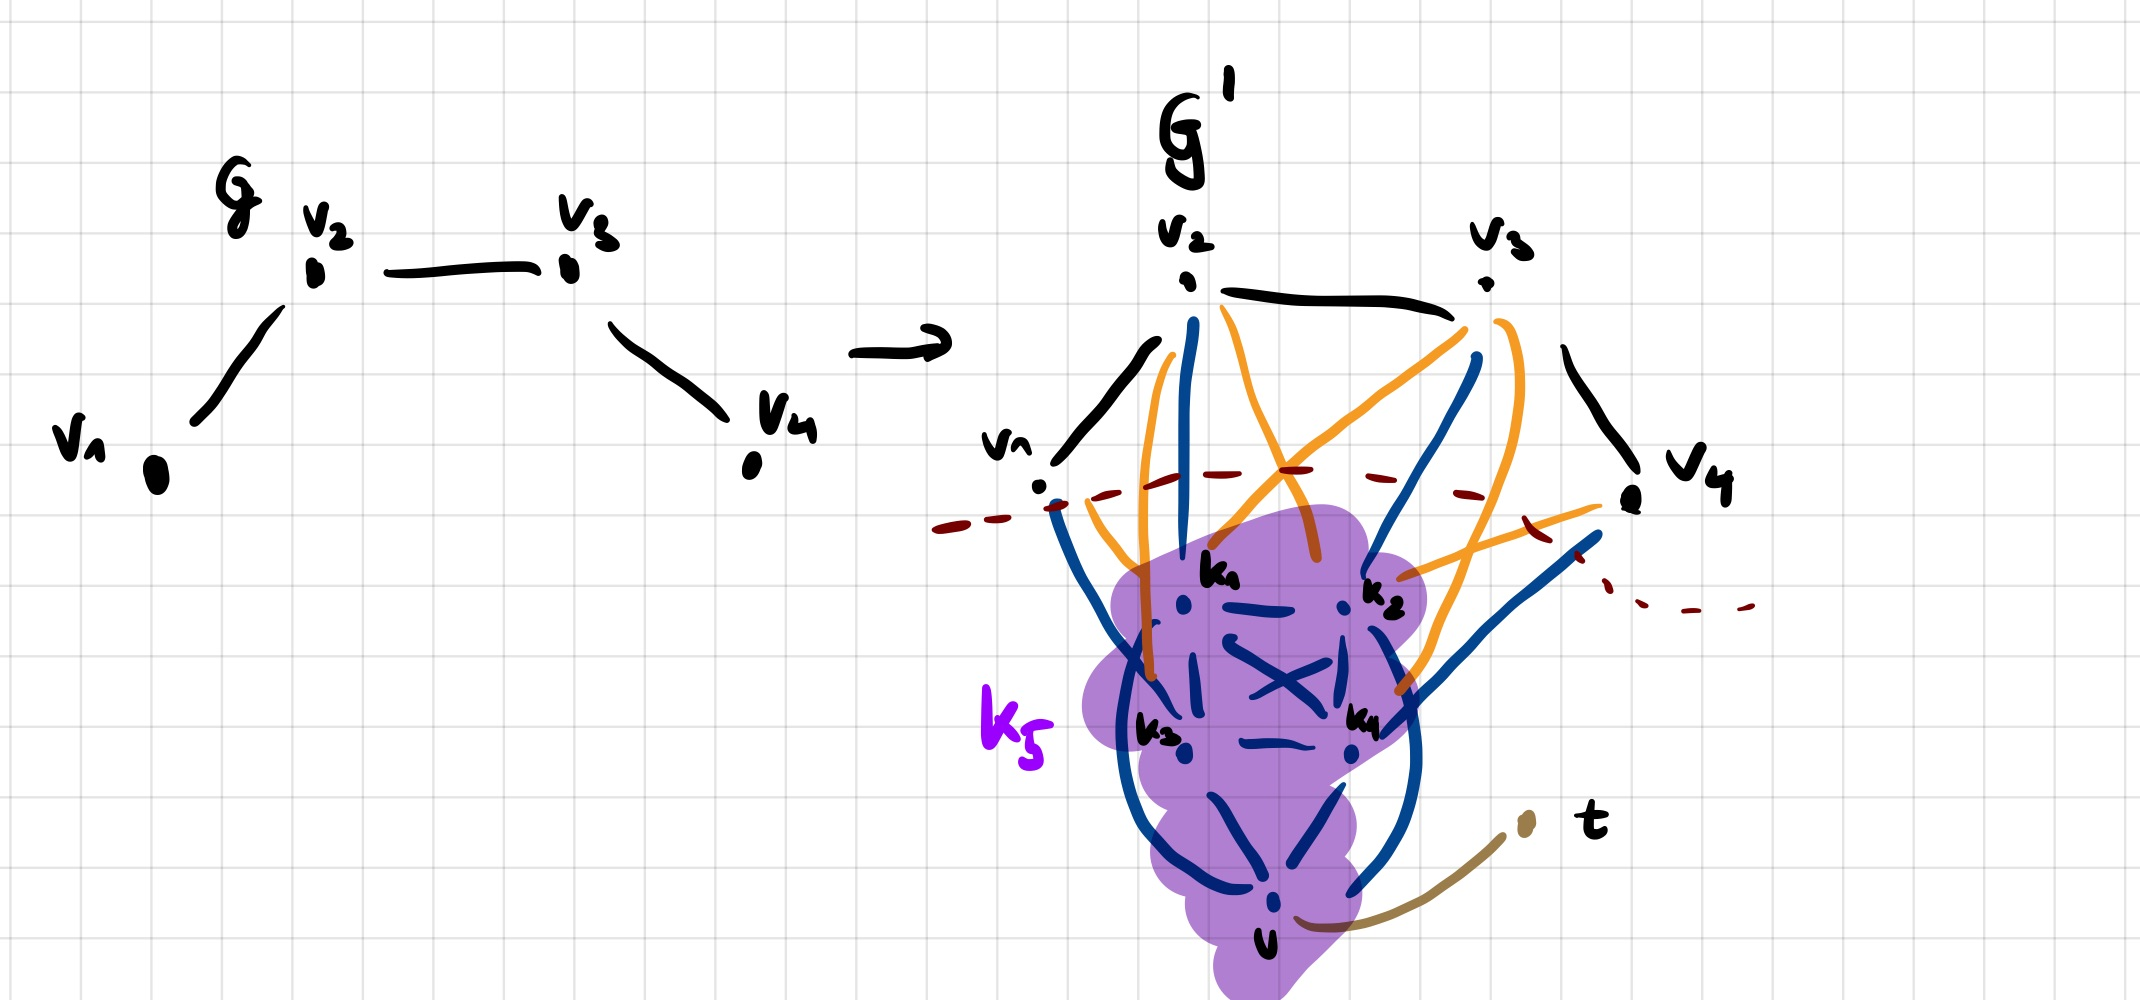
\includegraphics[scale=0.16]{pages/img/construct-chordal-reduction.jpg}
    \centering
    \caption{Constructing $G'$ by adding a $K_5$ and the vertex $t$}
    \label{fig:construct-chordal-reduction}
\end{figure}

\begin{proof}
    

    Given a chordal graph $G = (V = \{v_1,...,v_n\}, E)$, we construct a chordal graph G' as described below (See also fig \ref{fig:construct-chordal-reduction}):
    \begin{enumerate}
        \item Add a $K_{n+1}$ consisting of the vertices \{$k_1,...,k_n,u\}$ and add an edge $(v_i, k_i)$ to each vertex $v_i$ of G. One vertex $u$ in the clique will remain untouched.
        \item Add one additional vertex $t$ and connect it with $u$.
        \item For all vertices $v_i$ in G, add a new edge $(n, k_i)$ for all $n \in N(v_i)$.
    \end{enumerate}



    \begin{corollary}\label{cliqueNeighbor}
       $N(v_i) \in G$ forms a clique iff $N(v_i)$ forms a clique in $G'$
    \end{corollary}

    \begin{subproof}

\begin{figure}[th]
    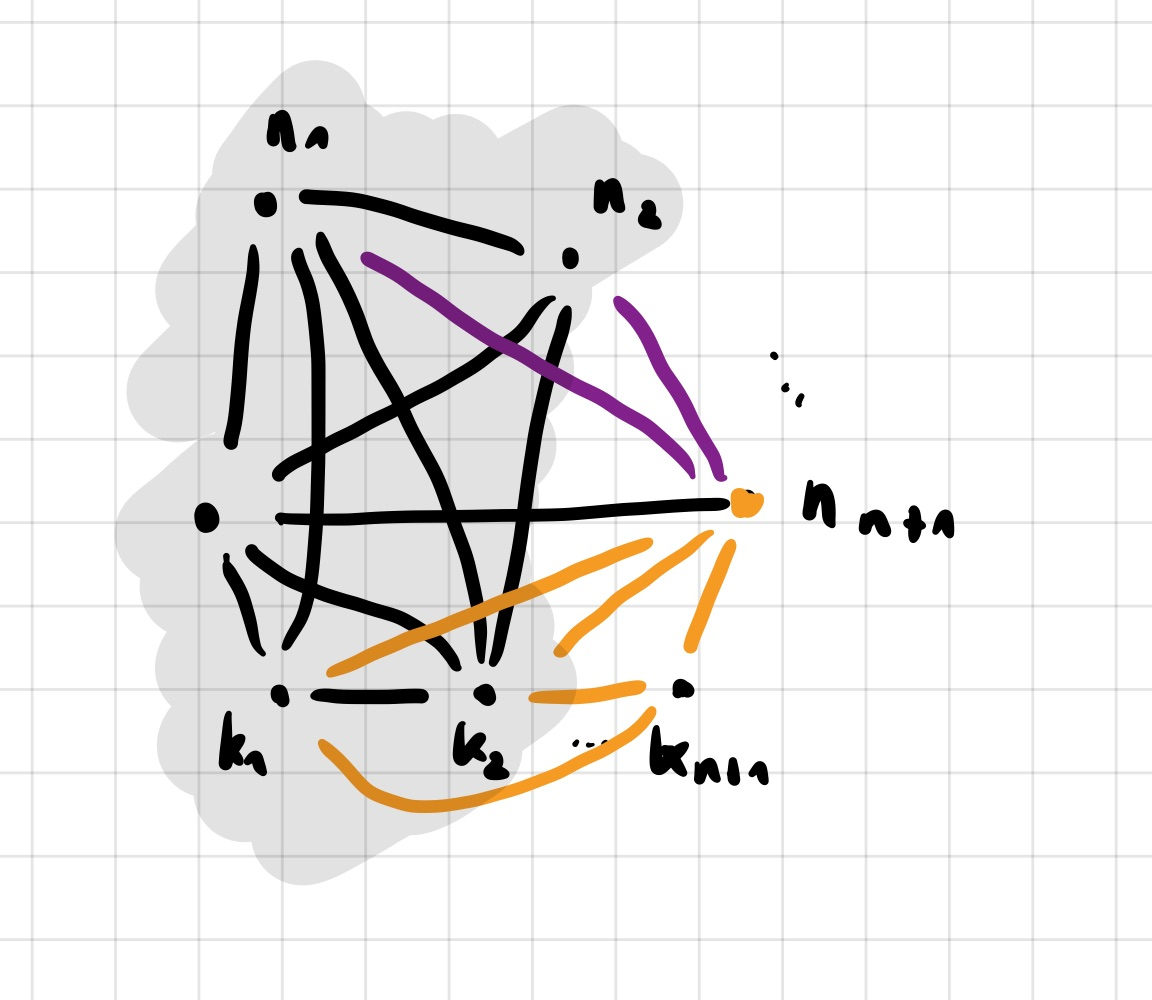
\includegraphics[scale=0.15]{pages/img/induction-step.jpg}
    \centering
    \caption{Induction Step}
    \label{fig:induction-step}
\end{figure}
        Asuming that $N(v_i)$ forms a clique in G, we show that it also forms a clique in G' by induction over the number of neighbors $z = abs(N(v_i))$ in G.

        \begin{itemize}
            \item $z = 0$: Holds trivially as we do not have a neighbor in G and in G' the connected $k_i$ forms a $P_1$, hence a clique.
            \item $z = z + 1$: 

            By IH, we already know that all neigbors $n_1,...,n_z$ form a clique together with their vertices in $k_{i}$. As $k_{z+1}, v_{z+1} \in N(v_i)$ now also in G', we show that $N(v_i)$ still forms clique in G'.

            Let $k_i$ be the vertex that was connected with $n_i$ during step 1. All we have to show is that $v_{z+1}$ and $k_{z+1}$ extend our previous clique, hence are fully connected with $N(v_i)$.
            
            $v_{z+1}$ connects to $N(v_i)$ in G by assumption. By our construction, there exists an edge to $k_1,...,k_z$, because we add an edge $(n_{z+1}, k_i)$ if there is an edge from $(n_{z+1}, n_i)$. (See fig \ref{fig:induction-step})

            $k_{z+1}$ form a complete subgraph with the other $k_i$ and is connected to all $n_i$ by construction because the edge $(n_{z+1},n_i)$ exists.  

            %Furthermore, $v_i$, $k_i$, $v_{n+1}$ and $k_{n+1}$ also form a clique, because we know that the edge $(k_i, k_{n+1})$ exists as both lay in the constructed complete induced subgraph and cross-wise edges exist from $(v_i, k_{n+1}) $ and $(v_{n+1}, k_i)$ by definition. Furthermore, $k_i$ is connected with all $N(v_{n+1})$, because $v_{n+1}$ is also a neighbor of them and hence, they must be connected to $k_i$.

            Therefore, $N(v_i)$ will also form a clique in $G'$.
        \end{itemize}

        On the other side, if $N(v_i)$ forms a clique in G', the vertices of $N(v_i)$ in G form an induced subgraph of G', hence preserving the clique.
        
    \end{subproof}
   
    \begin{corollary}
    G is Chordal iff G' is chordal.    
    \end{corollary}
    \begin{subproof}
    $\Rightarrow$: Asume $G$ chordal. Then exists a total elemination order $o = (v_1, ..., v_n)$ in G where removing $v_j$ sequentially returns cliques in $N(v_i)$.
    Define $o' = (v_1, ..., v_n, k_1, ..., k_n, u, t)$. Applying corollary \ref*{cliqueNeighbor} states that $(v_1, ... v_n)$ always gives cliques in G and according to corollary \ref*{cliqueNeighbor} also in G'. As the rest is directly part of a clique in G' by definition with an additional vertex of degree 1, o' is a total elemination order for $G'$, hence G' chordal.
    $\Leftarrow$: Holds as o' is always a total elimination order in G' and removing the complete subgraph $K_{n+1}$ and $u$ gives a total elemination order in G.
    \end{subproof}


    \begin{corollary}
    G has a Dominating Set of size k iff $G'$ has a dominating set of size $k+1$
    \end{corollary}
    \begin{subproof}
    Asume a Dominating Set D of size k in G. $D \cup \{u\}$ is a Semitotal Dominating Set in G' of size k + 1, because $u$ dominates $t$ and for each $v \in DS: d(v, u) \leq 2$.

    Contrary, asume a Semitotal Dominating Set $SD$ in $G'$. In order to dominate $t$, $u \in SD$ must hold, hence already dominating the complete subgraph $K_{n+1}$. If a vertex $k_i \in SD$, we exchange it with $v_i$ still preserving a Dominating Set. Taking $D = SD - \{ u \}$ gives our desired Dominating Set of size k.
    \end{subproof}
    As this reduction runs in FPT time and the parameter is only bounded by a function of k, this is a FPT reduction. As Dominating Set on Chordal Graphs is $w[2]-hard$, so is SDS on Chordal Graphs.

    %TODO partial elemination order
%    \begin{corollary}
%    SDS is $w[2]$ hard on Chordal Grpahs 
 %   \end{corollary}
\end{proof}

\subsection{\hmath $W[2]$-hard on Split Graphs}

\chapter{Open Questions and Further Research}

\vspace*{-50pt}

\begin{figure}[ht]
        
\includegraphics[width=0.35\textwidth, right]{img/placeholder.png}
        \captionsetup{textformat=empty,labelformat=blank}
        \caption{Generated with Dall-E. \url{https://labs.openai.com/}. ``A duck dominating sitting on a searose''}
\end{figure}

\epigraph{\itshape Todo select another quote}{Lewis Caroll, \textit{XXXX}}

* Chordal Bipartite Grap hs a very interesting case.
* Improve the Kernel Bound

